\setcounter{chapter}{4}
\chapter{Modelling}
\label{chap:modelling}
% 
% \markus{This is an example.}
% 
Nerve fiber modelling is a unique technique often used in simulations like \ac{dMRI}-simulations \dummy{}.
However, most \ac{dMRI} simulation tools use fast numeric simulation techniques like \dummy{}.
These use analytical functions to describe the fiber paths in order to calculate very quickly and accurately.
Current algorithms are able to use spline functions for single nerve fibers or fiber bundles \cite{Balls2009}.
Recently, with the improvement of computer performance and algorithms, simulation techniques such as Monte Carlo \dummy{} are used.
These simulate the random movement of individual water molecules within a volume.
If the target are \ac{WM} phantoms nerve fibers can be modelled as a meshed tube.
If \ac{WM} phantoms are involved, nerve fibers can be modeled as a meshed tube.
These have the advantage that any complex configuration can be modeled \eg{} fibers \dummy{}.
\\
%
A disadvantage, however, is that realistic model sizes require individual nerve fiber models in the order of $\SI{1}{\micro\meter}$.
Experimental \ac{dMRI} system have voxel sizes in the range of $\SIrange{100}{1000}{\micro\meter}$.
This means that for a signal the number of triangles in the mesh is quite large [\dummy{}].
Another challenge is to build a geometric configuration where no nerve fibers overlap (\ie{}, take the same volume in space).
\\
% 
Collision detection plays an important role in this process.
While other simulations that use geometric models (\eg{} protein folding \dummy{}) may use something like electric potentials where the actual geometric boundary is not so important.
In the case of \ac{3D-PLI} (and \ac{dMRI}) it will be shown to be different.
\\[\baselineskip]
% 
The following procedures are described in this chapter:
\begin{itemize}[nosep]
    \item geometric representation of the nerve fiber (bundle)
    \item user-friendly construction methods of models
    \item how to ensure collision-free models
\end{itemize}
% 
All described methods can be used within the package \pymodule{fastpli.model}:
% 
\begin{itemize}[nosep]
    \item \pymodule{sandbox}
    \item \pymodule{solver}
\end{itemize}
% 
The first module \pymodule{sandbox} contains routines that help the user to create simple geometric configurations.
These can then be used to build more complex structures of nerve fiber bundles.
The second module \pymodule{solver} contains a \cpp{} framework wrapped in a \python{} class to allow the user to build simpler \ac{API} (see \dummy{}).
\\
% 
First, however, it must be decided how a nerve fiber and a nerve bundle is to be represented.\todo{veroffentlichung in intro}
% 
% 
% 
\section{Nerve fiber representation}
\label{sec:nerve_fiber_representation}
% 
As described in \cref{sec:fiberArchitecture} \ac{WM} consist of densely packed bundles of nerve fibers.
Nerve fibers in \ac{WM} consist of axons surrounded by myelin (see \cref{fig:nerveFiber}).
The myelin is further split into several parts separated by Ranvier nodes to allow the spread of an action potential.
In the central nervous system, myelin is produced by olegodendrocytes, i.e. cells that wrap their small \say{arms} around locally adjacent axons.
The wrapping substance is called myelin and consists mainly of a lipid (fat) substance.
The question is how this tissue can be modelled and represented.
\\
% 
The main focus of modeling is to ensure that these models can be used for \ac{3D-PLI} simulations.
However, it is reasonable that these models can also be used for other tasks \eg{} for \ac{dMRI} simulations.
% 
\paragraph{What means usable?}
Since simulations are used, computer algorithms must be able to receive an input for a geometric fiber architecture.
One possibility is to look into the field of visualization techniques.
There, objects of different shapes have to be represented so that the computer algorithm can use the representation to visualize an image of the objects.
An obvious model for a fiber is a tube.
Usually objects like tubes are visualized with a surrounding mesh.
Meshes have the advantage that a texture can be applied to the surface.
However, since meshes usually consist of 3D triangles, this means a lot of points, \ie{} data and memory, for a good approximation to represent a model.
But even in the visualization domain tubes are not modeled from initial meshes.
They are initialized by a trajectory, which is then given an additional radius to obtain a volumetric representation.
This representation can also be used for nerve fiber tissue.
\\
% 
Existing simulation techniques \dummy{} allow to represent such structures as analytical mathematical objects \eg{} a parametric function $f(t) -> (x,y,z,r)$ with $(x,y,z)$ as 3D coordinate and $r$ as radius.
However, this drastically restricts the use of this function, since the user needs to know a parametric function in advance.
For trivial structures such as parallel straight fibers this is quite easy and fast to process.
However, if we want to model more complicated fabrics like densely interwoven fiber bundles, the task is almost impossible.
One possibility would be not to care if two fibers overlap, \ie{} occupy the same space in the volume.
This is done \eg{} for simulations such as protein folding, where the main interaction comes from electrodynamic forces.
However, it has already been shown that for more complicated \ac{3D-PLI} Simulations non-overlapping fibers are essential [\dummy{}].
\\
% 
For this reason, it was decided to represent fibers in such a way that they can be easily checked later whether colliding objects, \ie{} nerve fibers, are present.
\\
% 
\begin{figure}[!t]
    \centering
    \setlength{\tikzwidth}{0.75\textwidth}
    \inputtikz{gfx/model/conical_capsule_bb}
    \tikzset{external/export=false}
	\caption[cc and co]{\Acf{CC}: \raisebox{.25em}{\tikz \draw[black](0,0)--(0.275,0);} \ac{CC}, \raisebox{.25em}{\tikz \draw[blue, dash pattern=on 2.5pt off 2.5pt](0,0)--(0.275,0);} capsule, \raisebox{.25em}{\tikz \draw[red, dash pattern={on 2.5pt off 0.9pt on 0.42pt off 0.9pt}](0,0)--(0.275,0);} bounding box}
	\label{fig:conical_capsule}
\end{figure}
% 
\begin{figure}[!t]
    \centering
    \setlength{\tikzwidth}{0.5\textwidth}
    \inputtikz{gfx/model/capsule}
	\caption{schematic capsule}
	\label{fig:conical}
\end{figure}
% 
In order to enable any level of detail, a tubular fiber can be divided into a number of segments.
Each tubular segment can then be approximated as a cylindrical object.
However, since the radius of the nerve fibers can vary quite a lot along their path, the tube (or the fiber segments) must also be allowed to change.
If this is done via a cylindrical approximation, the boundary effects between two segments can lead to an unusual appearance/behavior.
It was therefore decided to approximate a fiber segment with a \ac{CC}, a 3D cone on which end spheres with the required radii are attached (see \cref{fig:conical_capsule}).
This has the advantage that between two fiber segments there is a smooth transition along the fiber axis (for reasonable curvature) (see \cref{fig:fiberReb, fig:modelLength}).
% 
\begin{figure}[!t]
    \setlength{\tikzwidth}{0.85\textwidth}
    \centering
    % \tikzset{external/export next=false}
    \inputtikz{gfx/model/fiber_model}
	\caption[]{Representation of a nerve fiber from a list of spheres.}
	\label{fig:fiberReb}
\end{figure}
% 
A nerve fiber can therefore be represented as a list of 4d coordinates (or spheres) (see \cref{fig:fiberReb}):
% z
\begin{align}
\begin{split}
% \vv{p} &= (x_i,y_i,z_i) \mid x,y,z \in \mathbb{R}\\
% r &\mid r \in \mathbb{R}\\
\mathit{fiber} &= \left\{ \vv{p}_i=(x_i,y_i,z_i), r_i \mid x,y,z \in \mathbb{R}, \, r \in \mathbb{R^+}, \, i \in \{0,1,...,N_{\mathit{points}}-1\}\right\} \\
\mathit{fiber\_segment}_i &= (\vv{p}_i, \vv{p}_{i+1}, r_i, r_{i+1}), \, i \in \{0,1,...,N_{\mathit{points}}-2\}
\end{split}
\end{align}
% 
\section{Sandbox}
% 
Since the geometrical representation of the fibers is defined, the question arises how such fibers can be constructed.
For this purpose the \ac{fastPLI} module \pymodule{fastpli.model.sandbox} was developed.
It contains a variety of methods that allow the user to create complex phantoms with fast construction algorithms.
\\
% 
These algorithms can be divided into two parts.
This toolbox focuses on constructing phantoms for the \ac{WM}.
Since \ac{WM} nerve fiber bundles are usually combined to nerve fiber bundles (see \dummy{}), the \pymodule{sandbox} module contains two main parts, which can contain exactly such structures.
%
Representation of nerve fiber bundles is very similar to that of nerve fibers: tube-like structures that are equipped with individual nerve fibers.
Representation of tubular structures has already been achieved (see \cref{sec:nerve_fiber_representation}).
\\
If nerve fiber bundles are imagined as a trajectory through the 3D coordinate systems, we can use the same Representation as for nerve fibers.
In addition, the radii contained can be used to scale a nerve fiber along its trajectory, i.e. inflate it.
\\
% 
The question remains how to populate such bundles.
To populate a trajectory, we can use a similar approach as in tractography (see \cref{sec:fillBundle}).
Starting with seed points at the beginning of the bundle.
\todo{improve transition}
% 
\subsection{Seeding fiber bundles}\label{sec:seeds}
% 
\begin{figure}[!t]
    \def\tikzheight{0.25\textwidth}
    \centering
    \subcaptionbox{\label{fig:triGrid}equilateral triangle grid}[.295\textwidth]{
    \inputtikz{gfx/model/triangular_grid}\hfill}
    \subcaptionbox{\label{fig:rndGrid}random grid}[.295\textwidth]{
    \inputtikz{gfx/model/rnd_circle_points}}\hfill
    \subcaptionbox{\label{fig:crossBundle}populated fiber bundles}[.39\textwidth]{
    \inputtikz{gfx/model/crossing_bundle}}
	\caption{Populating fiber bundles with seed points.}
% 	\label{fig:}
\end{figure}
% 
Seed points are stored as a list of 3D points:
\begin{align}
\mathit{seeds} = \left\{ \vv{p}_i=(x_i,y_i,z_i) \mid x,y,z \in \mathbb{R} , \, i \in \{0,1,N_{\mathit{seed\_points}}-1\}\right\}
\end{align}
% 
In order to form particularly dense fiber bundles, a method for generating an isosceles triangular grid was implemented.
Mathematically, a 2d packed circle contains the maximum packing density when arranged in a triangular grid\footnote{also referred to as hexagonal grid} for circles with equal radii (see \ref{fig:triGrid}).
However, this highly regular symmetrical grid can lead to strange results as will be shown later (\eg{} maxwell, simplified).
\todo{why rnd necesarry -> see simulation}
It should therefore only be used as an initial configuration. 
The positions can easily be changed.
A useful method was to add a boundary value to the initial starting points, \eg{} $\mathit{shift} = norm(0,\sigma)$.
However, since the initial configuration is often unknown, it is probably best to choose a random distribution (see \cref{fig:rndGrid}).
For a circle, this is done using:
\begin{equation}
\begin{aligned}
 \varphi &= \mathrm{uniform}(0,2 \pi) \hspace{4.2ex} && x = r \cos(\varphi)\\
 r &= R \sqrt{\mathrm{uniform}(0,1)} && y = r \sin(\varphi)
\end{aligned}
\end{equation}
% 
\subsection{Populating fiber bundles}\label{sec:fillBundle}
% 
\begin{figure}[!t]
    \centering
    \subcaptionbox{\label{fig:torsionCurve}Torsion along trajectory. The 
	\textcolor{green!50!black}{binormal}, \textcolor{red}{principal normal} vector and \textcolor{blue}{tangent vector} vector at each step are also the coordinate system for the seed points.}[.5\textwidth-4.3pt]{
    \setlength{\tikzwidth}{0.5\textwidth - 4.3pt}
    \inputtikz{gfx/model/min_torsion}}\hfill
    % 
    \subcaptionbox{\label{fig:filledBundle}Bending fiber along trajectory $f(t) = \left(\cos(t), \sin(t), 0 \right)$}[.5\textwidth-4.3pt]{
    \resizebox{.5\textwidth-4.3pt}{!}{
    \includegraphics{dev/gfx/circle_bundle.png}}}
	\caption{}
% 	\label{fig:}
\end{figure}
% 
To populate a nerve fiber bundle, the same idea is used as in tractography.
There seed points are initialized and then \dummy{} methods are used to calculate the next step.
However, we do not need to calculate the next step, because it is already defined by its trajectory.
But the bending of the bundle has to be considered.
\\
% 
There are already various techniques available.
A common one is the use of torsion of the curve. This is achieved by the following method:
% 
\begin{align}
\begin{split}
\vv{f}(s) &= (x(s),y(s),z(s)) \\
\vv{t}(s) &= \vv{f}\,'(s) \\
\vv{n}(s) &= \frac{\vv{t}\,'(s)}{|\vv{t}\,'(s)|} = \frac{\vv{r}\,''(s)}{|\vv{r}\,''(s)|} \\
\vv{b}(s) &= \vv{t}(s) \times \vv{n}(s),
\end{split}
\end{align}
% 
where $\vv{f}(s)$ is a parameterized trajectory of the parametric variable $s$, $\vv{t}(s)$ is the tangential vector, $\vv{n}(s)$ is the principal normal vector and $\vv{b}(s)$ is the binormal vector (see \cref{fig:torsionCurve}).
One could use this idea to rotate the seed points into the coordinate system of $\vv{t}(s),\vv{n}(s),\vv{b}(s)$.
However, this can lead to an arbitrary rotation of the fibers, \eg{} if the curve is described in such a way that $\vv{n}(s),\vv{b}(s)$ would continuously rotate around $\vv{t}(s)$.
\\
% 
Since it is plausible that nerve fiber bundles would not do this, a different approach was chosen.
The idea is to minimize the rotation from one step to the next step.
When defining a plane, within the vectors $\vv{n}(s),\vv{b}(s)$ defined above, the plane is rotated from one step $i$ to the next step $i+1$ by the same amount by which the curve bends.
However, the rotation along the vector $\vv{t}(s)$ should be $0$.
Since a discrete point exists, the plane can be rotated by the same amount as the vector $\vv{t}(s)$.
However, to obtain a plane in the center of the points $\vv{p}_{i-1}, \vv{p}_{i}, \vv{p}_{i}, \vv{p}_{i+1}$ the middle orientation of these points will be used.
An example is shown in \cref{fig:filledBundle}.
\\
\todo{explain and check algorithm}
% 
Now the bundle can easily be populated by starting at the beginning of the fiber, placing the seed points at the starting point and rotating the seed point for each step $i$ along the trajectory by rotating only along a vector perpendicular to the bend of the curve.
% 
\subsection{cube models} \label{sec:cubeModelBuilding}
% 
\begin{figure}[!t]
    \centering
    \setlength{\tikzwidth}{0.5\textwidth}
    \inputtikz{gfx/model/cube_build}
	\caption{Populating a cuboid with straight fibers initialized by seed points along the direction $\vv{v}$.}
    \label{fig:cubeBuild}%
\end{figure}
% 
To be able to create a model with a main fiber orientation, a method was also developed to populate a cuboid volume.
This method allows to create fibers within the cuboid volume that are oriented along a user-defined main orientation $\vv{v}$ (see \cref{fig:cubeBuild}). 
The individual fibers are also initialized with seed points.
An infinite line with the main orientation $\vv{v}$ is laid through each seed point.
If a line collides with the volume, the line inside the cube is returned as a fiber.
% 
\subsection{cylindric models}
% 
\begin{figure}[!t]
    \centering
    \setlength{\tikzwidth}{0.31\textwidth}
    \subcaptionbox{\label{fig:cylCircular}%
        Circular population.
    }[.33\textwidth-1ex]{
    \inputtikz{gfx/model/cylinder_circular}}\hfill
    % 
    \subcaptionbox{\label{fig:cylRadial}%
        Radial population.
    }[.33\textwidth-1ex]{
    \inputtikz{gfx/model/cylinder_radial}}\hfill
    % 
    \subcaptionbox{\label{fig:cylParallel}%
        Parallel population.
    }[.33\textwidth-1ex]{
    \inputtikz{gfx/model/cylinder_parallel}}
	\caption{Populating of cylindrical objects. The green area shows the area corresponding to the seed points xy-plane. The coordinate system \textcolor{red}{red} indicates the coordinate origin for the seed points.}
% 	\label{fig:}
\end{figure}
% 
Finally, a method for building cylindrical structures was implemented.
Since a cylinder has three \say{symmetries}, all three were implemented to provide an option to populate the volume.
First we define the coordinate system.
The cylinder of an outer radius $r_{\mathit{out}}$ and an inner radius $r_{\mathit{in}}$ is oriented along the z-axis with a height $h$, starting at $(0,0,0)$.
Additionally, the cylinder can be cut radially from a directional angle $\alpha$ to $\beta$.
% 
\paragraph{a) circular} mimics a path on the $xy$ level of a cylinder (see \cref{fig:cylCircular}).
The seed points are used along the surface of the cross section, starting at the first $\alpha$ direction angle.
From there, the fiber runs in a circular pattern to the second directional angle $\beta$.
The step size of the circular path can be changed.
% 
\paragraph{b) radial} cylindrical fibers are oriented from the center of the $xy$ plane to the outside of the cylinder (see \cref{fig:cylRadial}).
The seed points are located along the inner radial plane.
Thus, the fiber density decreases along its path.
Here, the shape is also only populated inside the boundaries of the radii and angles.
% 
\paragraph{c) parallel} fibers are oriented along the cylinder (see \cref{fig:cylParallel}).
Here the seed points are located in the $xy$-plane (see \cref{fig:cylParallel}). Only fibers that collide with the cylinder are used. The borders are unchanged.
% 
% 
% 
\section{Solving fiber collisions}
\label{sec:Solver}
% 
A major disadvantage of all previous methods is that the user has to make sure that his fiber path leaves enough space so that the fibers (paths + radii) have enough room and do not overlap.
This can be achieved for fibers with constant radii along their course in the upper designs.
However, for more complex structures, \eg{} crossing fiber bundles, this is almost impossible.
Therefore, a method has been developed that takes the user-defined fibers and checks for collisions.
If a collision is found, it will try to move the colliding objects slightly apart so that the collision starts to disappear.
\\
% 
This concept is quite simple.
Collision detection algorithms have been used for centuries, especially in the gaming environment where \eg{} a character should not be able to walk through a wall.
Another wide range of algorithms is used in visualization.
There the problem is usually to detect the collision between a light path (mathematical line) and an object, usually a triangular surface.
Also known as raytracing.
The disadvantage in both areas is that the computing time is limited.
Therefore, algorithms there use abbreviations that come as close as possible to reality, but still produce useful data \eg{} in computer games it is very important to have a stable framerate of over 60 \ac{fps} (or with current technology even over 120 \ac{fps}).
For the gaming experience, however, it is not important whether the character can easily run against an object or not.
Therefore an object could be approximated like a stone by a sphere(s).
\\
%
But since here the goal is to create models that are as large, complex and precise as possible, a new algorithm has to be developed that is specialized in this task.
% 
\\[\baselineskip]
\todo{next sections as subsections?}
%
\section{World/main}
% 
\begin{lstfloat}[!tb]
\lstset{style=python}
\begin{lstlisting}[]
def step():
    # Reset Parameter
    SetSpeed(objects, 0)
    
    # Building Octree
    octree = Octree(objects)
    
    # Collision Detection
    for leaf in octree:
        colliding_objs = CheckLeaf(leaf.fiber_list)
        colliding_list.insert(colliding_objs)
	
    # Seperation Process
    AddSpeed(colliding_list)
    NormalizeSpeed(colliding_list)
    MoveObject(colliding_list)
	
    # Shape Control
    SegmentLength(colliding_list, target_length)
    BendingRadius(colliding_list, target_curvature)

    return colliding_list.is_empty()
\end{lstlisting}
\caption{Pseudocode of the \code{main} algorithm: The function \code{FiberCollisionSolver} will loop the followings four steps, which are run in parallel, until no collision are detected anymore: 1. build an \code{octree} from all objects, 2. \code{Collision Detection}, 3. \code{Seperation Process} and 4. \code{Shape Control}. \itodo{check algorithm, spetially movement phase}}
\label{alg:pseudocode_solver}
\end{lstfloat}
% 
The world/main function is the \code{loop}, which is executed to calculate the collision, move the objects and check the boundary collision (see \cref{alg:pseudocode_solver}).
The loop procedure is similar to a game loop or a visualization loop (\eg{} in glut \code{glutMainLoop}).
But to give the user as much control as possible, the user has to go through each step in a separate loop like in one of the examples within the packages.
After each step, the user is now able to change parameters, fiber paths, add/remove fibers from the \say{scene} and so on.
In addition, the user can decide whether a completely solved volume is required and e.g. break out of the loop before the final step (see \dummy{}).
%
A stand alone Algorithm is already publish in \cite{Matuschke2019}.
At this point it is integrated inside the \ac{fastPLI} package under \pymodule{fastpli.model.solver}.
Before going into the details of the algorithm, the collision detection algorithm is described.
% 
% 
% 
\subsection{Collision Detection}
\label{sec:collisionDetection}
% 
\begin{lstfloat}[!t]
\resizebox{\textwidth}{!}{
% \begin{sideways}
\begin{tabular}{|cc|cc|}
\hline
\hspace{1em} &
\begin{minipage}{0.4625\textwidth}
\lstinputlisting[style=cpp,basicstyle=\scriptsize\ttfamily,firstline=1,lastline=32]{code/collision_detection.py}
\end{minipage} & \hspace{1em} &
\begin{minipage}{0.4625\textwidth}
\lstinputlisting[style=cpp,basicstyle=\scriptsize\ttfamily,firstline=33,lastline=64,firstnumber=35]{code/collision_detection.py}
\end{minipage} \\
\hline
\end{tabular}
% \end{sideways}
}
\caption{Collision detection between two capsule objects. The distance as well as the points on the line segments is returned. A collision takes place if the distance is smaller than $\mathit{cone_a.r}+\mathit{cone_b.r} > d$.}
\label{alg:pseudocodeCollisionDetection}
\end{lstfloat}
% 
As described in \cref{sec:nerve_fiber_representation}, nerve fibers are represented as a chain of spheres, where two adjacent spheres are combined to form a fiber segment that has a \ac{CC} (see \cref{fig:conical_capsule}).
% 
Therefore an algorithm is necessary to calculate a collision between up to \ac{CC}.
This is a non-trivial task and very computationally intensive.
Therefore it was decided to change the object representation for the collision detection part from a \ac{CC} to a capsule (see \cref{fig:conical_capsule}).
This means that the radii of the \ac{CC} for both spheres grow to the maximum of the two spheres $r_{\mathit{capsule}} = \mathrm{max}(r_0, r_1)$.
This has the disadvantage that at intersections of two adjacent cones the radii can actually be smaller, but if the change in radius is not rapid, this is acceptable.
\\
The algorithm for detecting collisions between two capsules is shown in \cref{alg:pseudocodeCollisionDetection}\footnote{\href{https://www.john.geek.nz/2009/03/code-shortest-distance-between-any-two-line-segments/}{https://www.john.geek.nz/2009/03/code-shortest-distance-between-any-two-line-segments/}}.
% 
It works on the principle that it calculates the shortest distance between two line segments.
Three cases can occur.
First, the shortest distance is a line perpendicular to two of the two line segments of the cones.
Second, only one line segment is perpendicular to the line of the shortest distance.
The other has an anchor point at either its first or second point.
Third, the shortest distance is a connection between one of the points of the two cones.
For cones, a collision occurs when the distance is smaller than the sum of the two radii.
\\
\begin{figure}[!t]
    \centering
    \def\tikzheight{0.5\textwidth}
    \inputtikz{gfx/model/shortest_dist}
	\caption{shortest distance}
	\label{fig:shortDist}
\end{figure}
% 
The problem with \ac{CC} is that as the radii along its axis change, it is no longer simply the case that the shortest distance between two line segments is also the shortest distance between a 3d \ac{CC}.
To do this, the lines on both object surfaces containing the closed point must be found.
However, this is very complex to calculate and was therefore rejected.
% 
It is expected that the calculation of the collision check will be the most costly function at this point.
Therefore the next logical step is to reduce the scope of the calculations as much as possible.
A first brute force collision check would check each object with all other objects.
The next object must then be checked with $n-1$ etc.
This results in a calculation effort of $\mathcal{O}(n^{2})$, which is not acceptable for large n.
To reduce the number of collision checks to be performed, an octree structure is used.
% 
\subsection{Octree}
% 
\begin{figure}[!t]
    \centering
    \subcaptionbox{\label{fig:octreeCube}octree}[.3\textwidth]{
    \def\tikzheight{0.6\textwidth}
    \inputtikz{gfx/model/oct_tree}}
    \subcaptionbox{\label{fig:collision2D}collision 2d}[.65\textwidth]{
    \def\tikzheight{0.6\textwidth}
    \inputtikz{gfx/model/collision_tree}}
	\caption{}
	\label{fig:octree}
\end{figure}
% 
A \name{tree} is a data structure that consists of a collection of \name{nodes} that are connected to each other.
A node is connected in the direction of the \name{root} with a single parent node and in the direction of the \name{branches} with several \name{children} or \name{branches}.
The nodes at the end of a branch are called \name{leaves}, which contain the data.
Traversing an evenly distributed tree has the advantage that the cost of the traversing it is $\mathcal{O}(\log(n))$.
\\
% 
An octree is a special kind of tree where each node contains eight children.
This allows to divide a cubic volume into eight equally cut sub-cubes.
An example is shown in \cref{fig:octreeCube}.
This means that the length of the volumes shrinks exponentially with $(1/2)^\mathit{level}$.
An octree can be implemented in different ways.
Here a recursion function was chosen (see \cref{alg:pseudocode_octree}).
% 
\begin{lstfloat}[!tb]
\lstset{style=python}
\begin{lstlisting}[]
def octree(volume, objects):
    if num(objects) > threshold:
        sub_volumes, sub_objects = split(volume, objects)
        leafs = [octree(v,o) for v,o in zip(sub_volumes, sub_objets)]
    else:
        leafs=[objects]
    return leafs
\end{lstlisting}
\caption{Pseudocode of octree}
\label{alg:pseudocode_octree}
\end{lstfloat}
% 
In computer science, a recursive function means that a function (can) call itself.
The idea is the following.
At the beginning all objects must be sorted into the eight leaves of the current node (if the number of objects is not trivial to small).
This means that for each object it must be checked whether there is a collision with one or more of the eight leaves.
However, since this already means a high test effort, the test function should be as fast as possible, usually approximate.
For this purpose only the \ac{AABB} of the object is checked if it collides with the sheet volume (which is its own \ac{AABB}) (see \cref{fig:collision2D}).
A collision detection of two \ac{AABB}s is rather simple (see \cref{alg:collisionAABB}).
% 
\begin{lstfloat}[!tb]
\lstset{style=python}
\begin{lstlisting}[]
def aabb_collide(aabb_0, aabb_1):
  for i in dim(aabb):
      if aabb_0[i].min > aabb_1[i].max:
         return false
      if aabb_0[i].max < aabb_1[i].min:
         return false
  return true
\end{lstlisting}
\caption{Pseudocode collision between aabbs.}
\label{alg:collisionAABB}
\end{lstfloat}
% 
When all objects are sorted into their respective sub-volumes, recursion can begin.
Since a branch can be considered a node, the same algorithm can be executed again until a desired limit or property is reached.
This means that the current (sub-)volume will be split into eight sub-volumes again, if necessary, and the objects of the current (sub-)volume will be sorted into the new sub-volumes.
The recursion also means that the next function call must contain a list of the current objects.
This means either that the objects must be copied, which is time-consuming, or they must be moved, which is also time-consuming depending on the structure, and they must be moved back, or a pointer or index must be traversed.
The last option was chosen because it proved to be the fastest in a speed test during the implementation process.
The next question is, which is the desired goal to stop the branching process and characterize the node as a leaf.
\\[\baselineskip]
% 
The goal is of course the reduction of the computing time.
However, this means that there is no simple answer for complex models and thus for unique octrees.
The usual way is to have the three following restrictions.
% 
\paragraph{Number of level limitation:}
The maximum number of steps is usually limited in the following two ways.
First, when a threshold value for the counter of the maximum number of levels is reached.
Since the since of the volume shrinks exponential, this is a good way to control the amount of calculations.
Usually, however, this is further limited by limiting the minimum size of the volume.
For a number of object sizes, this means that splitting into the next volume only makes sense if the object sizes are at least twice smaller than the current volume.
Otherwise, all eight volumes would contain all objects and the number of collision checks would increase by eight.
Since all objects are expected to be in the same order of magnitude, a global value can be set by first measuring the maximum \ac{AABB} and setting the threshold twice higher.
This automatically limits the maximum number of levels that can be reached.
% 
\paragraph{Minimal number of objects:}
The optimal minimum number of objects in a node to start the final collision algorithm must be measured, since it depends on the instructions actually executed on the system.
It is a trade-off between executing less computationally intensive, costly and highly accurate collision checks and executing at least eight more branches.
In the development phase of the algorithm this value was chosen as \comment{20}\dummy{}.
Of course the user can change this hard coded value if necessary. 
\\
% 
With the resulting list of colliding object pairs, the next task is to perform the separation process.
%
\section{Separation Phase}
To solve a collision between two \ac{CC} objects, each point $\vv{p}_i$ and $\vv{p}_{i+1}$ of both objects must be moved.
The movement is parallel to the smallest distance line between the two objects.
To take the 3D placement into account, the movement is weighted by the distance of each point from the intersection with the smallest distance line (see \cref{fig:shortDist}):
\begin{align}
v_i = \dummy{}
\end{align}
This leads to a more controlled movement if \eg{} only the two ends of the fiber objects collide.
\\
% 
TThe motion is stored as the sum of all collisions for each object in a velocity \code{std::vector}.
The maximum speed is limited to a value of $v_{\max} = 0.1 \times \min(\mathit{object radius})$.
This is limited due to two required properties. First, it prevents movement through another object and second, it smoothes the movement and thus the maximum achievable density of the resulting models.
However, this also means that the solution process takes more time.
\\
% 
A special case are the end points.
These are only allowed to move along the surface perpendicular to the first / last segment line.
This prevents the fibers from growing into infinity.
% 
\section{Shape Control}\label{chap5:ShapeControl}
The movement of individual points can lead to a distorted fiber model, \eg{} two points move very far apart.
Therefore boundary conditions must be specified.
It was decided to use the following two conditions.
% 
\subsection{Mean segment length}
% 
\begin{figure}[!t]
    \centering
    \setlength{\tikzwidth}{.45\textwidth}
    \subcaptionbox{merge}[.49\textwidth]{
    \inputtikz{gfx/model/model_merge}}
    \subcaptionbox{split}[.49\textwidth]{
    \inputtikz{gfx/model/model_split}}
	\caption{Length control for fibers $f$ and $f'$}
	\label{fig:mergeSplit}
\end{figure}
% 
% 
\begin{figure}[!t]
    \centering
    \setlength{\tikzwidth}{0.75\textwidth}
    \tikzset{external/export next=false}
    \inputtikz{gfx/model/model_length}
	\caption{different fiber segment length.}
	\label{fig:modelLength}
\end{figure}
% 
The mean segment length is the distance between the two points of an object.
If the segment length becomes too small/large, the points within a fiber corresponding to the object are merged/separated, adding one point less/one new point.
The minimum/maximum distance of the object is set to $d_{\min} = \frac{2}{3} \overline{d}, d_{\max} = \frac{4}{3}\overline{d}$.
Therefore the mean value of the object is:
\begin{align}
\frac{d_{\min} + d_{\max}}{2} = \overline{d}
\end{align}
% 
If a new point is created due to exceeding the maximum limitation, the new points $\vv{p}_{new}$ radius $r_{new}$ and velocity $\vv{v}_{new}$ are 
\begin{align}
\vv{p}_{new} = \frac{\vv{p}_{i} + \vv{p}_{i+1}}{2},\enspace
r_{new} = \frac{r_{i} + r_{i+1}}{2},\enspace
\vv{v}_{new} = \frac{\vv{v}_{i} + \vv{v}_{i+1}}{2}
\end{align}
% 
\subsection{Bending radius}
% 
\begin{figure}[!t]
    \centering
    \def\tikzheight{.40\textwidth}
    \subcaptionbox{Boundry segment length: lower bound $phi=\SI{60}{\degree} \xrightarrow{} r_{min} \geq \SI{0.5773}{} \cdot l_{mean}$}[.475\textwidth]{
    \inputtikz{gfx/model/model_circle}}\hfill
    \subcaptionbox{\label{fig:boundaryLength}Boundary segment radii: lower bound $r_{min} \geq \fiberRadiusMean $}[.45\textwidth]{
    \inputtikz{gfx/model/model_circular}}
	\caption{Geometrical boundry condition for fiber segment length \segLength and fiber bending radius \segRadius.}
	\label{fig:modelCircle}
\end{figure}
% 
The bending radius is defined as the circle radius corresponding to the circle defined by three adjacent points $\vv{p}_{i-1}, \vv{p}_{i}, \vv{p}_{i+1}$ (see \cref{fig:boundaryLength}). 
The limit is set as a minimum radius of $r_{\min}$.
If a $p_{i}$ point in a fiber falls below this value, the three points are moved.
$p_{i-1},p_{i+1}$ is moved \dummy{} and $p_{i}$ opposite each other.
This reduces the curvature.
\\
% 
\section{Movement Phase}
All movements are added to the velocity vector before performing the overall movement.
The algorithm performs each step sequentially (see \cref{alg:pseudocode_solver}).
% 
Finally a volume is marked as collision free, if no collision are found and all boundary conditions are fulfilled. 
The boundary conditions can be set to 0 to ignore them.
Additionally a drag value can be set, to reduce the velocity by its factor after each step.
It can help to reach a collision free volume faster, however the density will be significantly reduced.
Therefore the value is to 0 so that after each step the velocity is reset to $\vv{0}$. 
% 
\section{Optimization / Parallelisation}
% 
Among other techniques, two main optimisation techniques are used to speed up the process.
% 
\paragraph{Memory alignment}
The \code{std::vector} has the advantage that the data is linear in memory.
Modern \acp{CPU} have a built-in method called \say{ache prefetching}.
Data must be prepared and sent from the \ac{RAM} to the cache of the \acp{CPU}.
This takes time.
The main advantage of the cache is that it is very fast.
However, since it must be very close to the \ac{CPU}, the cache is very fast. (in modern systems the speed is already limited by the speed of light) its size is very limited (usually around $\si{\mega\byte}$).
The prefetcher is an ingenious directive, which not only obtains the item at address $i$ in memory, but also the item next to it ($i+1$ or $i-1$ depending on the algorithm).
Since many algorithms pass through arrays, the next item to be calculated is usually the next (or previous) item.
Therefore the time needed to copy the data into the cache and prepare it is reduced.
It can be shown that for linear operations on the memory the cache prefetcher reduces the time so much that it behaves as if the \ac{CPU} has an infinite cache.
% 
\paragraph{OpenMP}
% 
To be able to use several \acp{CPU}, \openmp is used. With a structure like an octree, the separation process into the new partial volumes can already be parallelized up to eight cores.
However, since all eight cores have to share the object list data, even if they are only reading, it is no longer possible from this point on to achieve up to eight times the speed (see later acceleration measurements \dummy{}).
\\
% 
Furthermore, all instructions containing loops, such as the separation phase, are also parallelized with \openmp.
% 
% 
% 
\section{Visualization}
% 
A visualization tool was written to visualize the fiber configuration.
This enables the user to get a direct feedback (\eg{} after each step) to adjust the initial fiber configuration or boundary condition.
It is written in \cpp{} and \opengl{} \cite{isocpp, khronos}.
\\
% 
\ac{CC} are rendered using the \code{gluCylinder} function provided by the \name{GLUT} library for a rough but fast visualization.
Representation and thus the collision check algorithm is also provided by the \name{GLUT} library for a rough but fast visualization.
For a more accurate and correct visualization of the \ac{CC} a self-implemented rendering was developed.
The first step in the visualization of surfaces is usually the generation of a \name{mesh} from triangles.
A texture can then be placed on each triangle.
Since fibers have to be visualized here, the mesh is generated as a tube surrounding the fiber with circularly arranged points around a fiber point $p_i$ (see \cref{fig:mesh}).
Corner points and normals are calculated from the mesh, which are finally rendered with a color within an illuminated scene.
To enable visualization of the inner axon, the myelin sheath can also be rendered.

% 
\begin{figure}[!t]
    \setlength{\tikzwidth}{0.5\textwidth}
    \subcaptionbox{\label{fig:mesh}mesh}[0.49\textwidth]{
    \inputtikz{gfx/model/vis_a}}
    \subcaptionbox{vis}[0.49\textwidth]{
    \inputtikz{gfx/model/vis_b}}
	\caption{Generating mesh for visualization.}
	\label{fig:vis_mesh}
\end{figure}
% 
\paragraph{Disclamer}
This is a fast implementation.
Current rendering software uses much more advanced techniques.
However, this rendering algorithm has been written to be an easily integrated tool that uses only the additional \name{OpenGl 2} and \name{GLUT} library.
\\
% 
A more advanced tool, the \name{FAConstructor} \cite{Reuter2019} was written by Andr'e Reuter as part of this doctoral thesis.
This tool uses \name{OpenGl 3} and additional calculation on the GPU. Additionally it allows a user-defined interactive technique to create a 3D fiber model.
The next step is already carried out with the visualization tool by Nicole Schubert called \name{PLIVis}.
% 
\subsection{Wall opacity}
% 
In order to visualize axons within the myelinated nerve fibers, the visualized vertices must be transparent.
However, this requires sorted vertices along the z-axis (viewer/camera? axis).
This is needed because vertices are rendered from back to front, so that the absorption of light can be taken into account.
This process takes a certain amount of time and is therefore only recommended for screen shoots at this time (see \dummy{}).
% 
% 
\vspace{5pt}
\hrule
\vspace{6pt}
% 
\newpage
% 
\section{Medusa}
% 
\itodo{Section neu schreiben. Bisher nur Ideen.}
% 
Additionally to the previous discussed modelling algorithm (see \cref{sec:Solver}), the \ac{MEDUSA} algorithm, was developed in a cooperation with the team Neurospin from \ac{CEA} in France \cite{Ginsburger2019}. The targed was to develop an algorithm which can build a library of \ac{WM} tissue. This library should not only contain nerve fibers, but also other cell types like olegodendrocites or astrocytes. These cell types are currently not used in \ac{3D-PLI} routine analysis however in \ac{dMRI} the cell are quite important [\dummy{}]. Furthermore these cells take up additional volume which results in different nerve fiber configurations.\\
% 
Since this tool aims to build a statistically library, other parameters are chosen for boundary conditions. These parameters are chosen as close as possible from the current \ac{dMRI} models:
\dummy{}\\
\dummy{}\\
% 
% Instead of choosing \ac{CC} the fibers and cells are represented as a collection of spheres. This has the advantage that the collision of spheres are more easier to be calculated:
% \begin{align}
%     d < r_i + r_j
% \end{align}
% 
On the other side more spheres are needed to represent a fiber. There can always be a resulting overlapp which depnding on the usecase, can lead to .. results.\\
% 
Cells are also represented as a collection of spheres, filling out the sum of the spheres volume. \\
%
In this theses cells are disregarded. A full description of the construction with astrocytes and olegodendrocytes can be found in \cite{Ginsburger2019}.
% 
\subsection{Algorithm}
% 
\begin{figure}[!t]
\centering
% \resizebox{0.75\textwidth}{!}{
\setlength{\tikzwidth}{0.75\textwidth}
\inputtikz{gfx/model/medusa/medusa_spheres}
% }
\caption{modified from \cite{Ginsburger2019}}
\label{fig:model:medusa_4}
\end{figure}
%
% \begin{figure}[!t]
%     \centering
%     % \resizebox{0.75\textwidth}{!}{
%     \setlength{\tikzwidth}{0.75\textwidth}
%     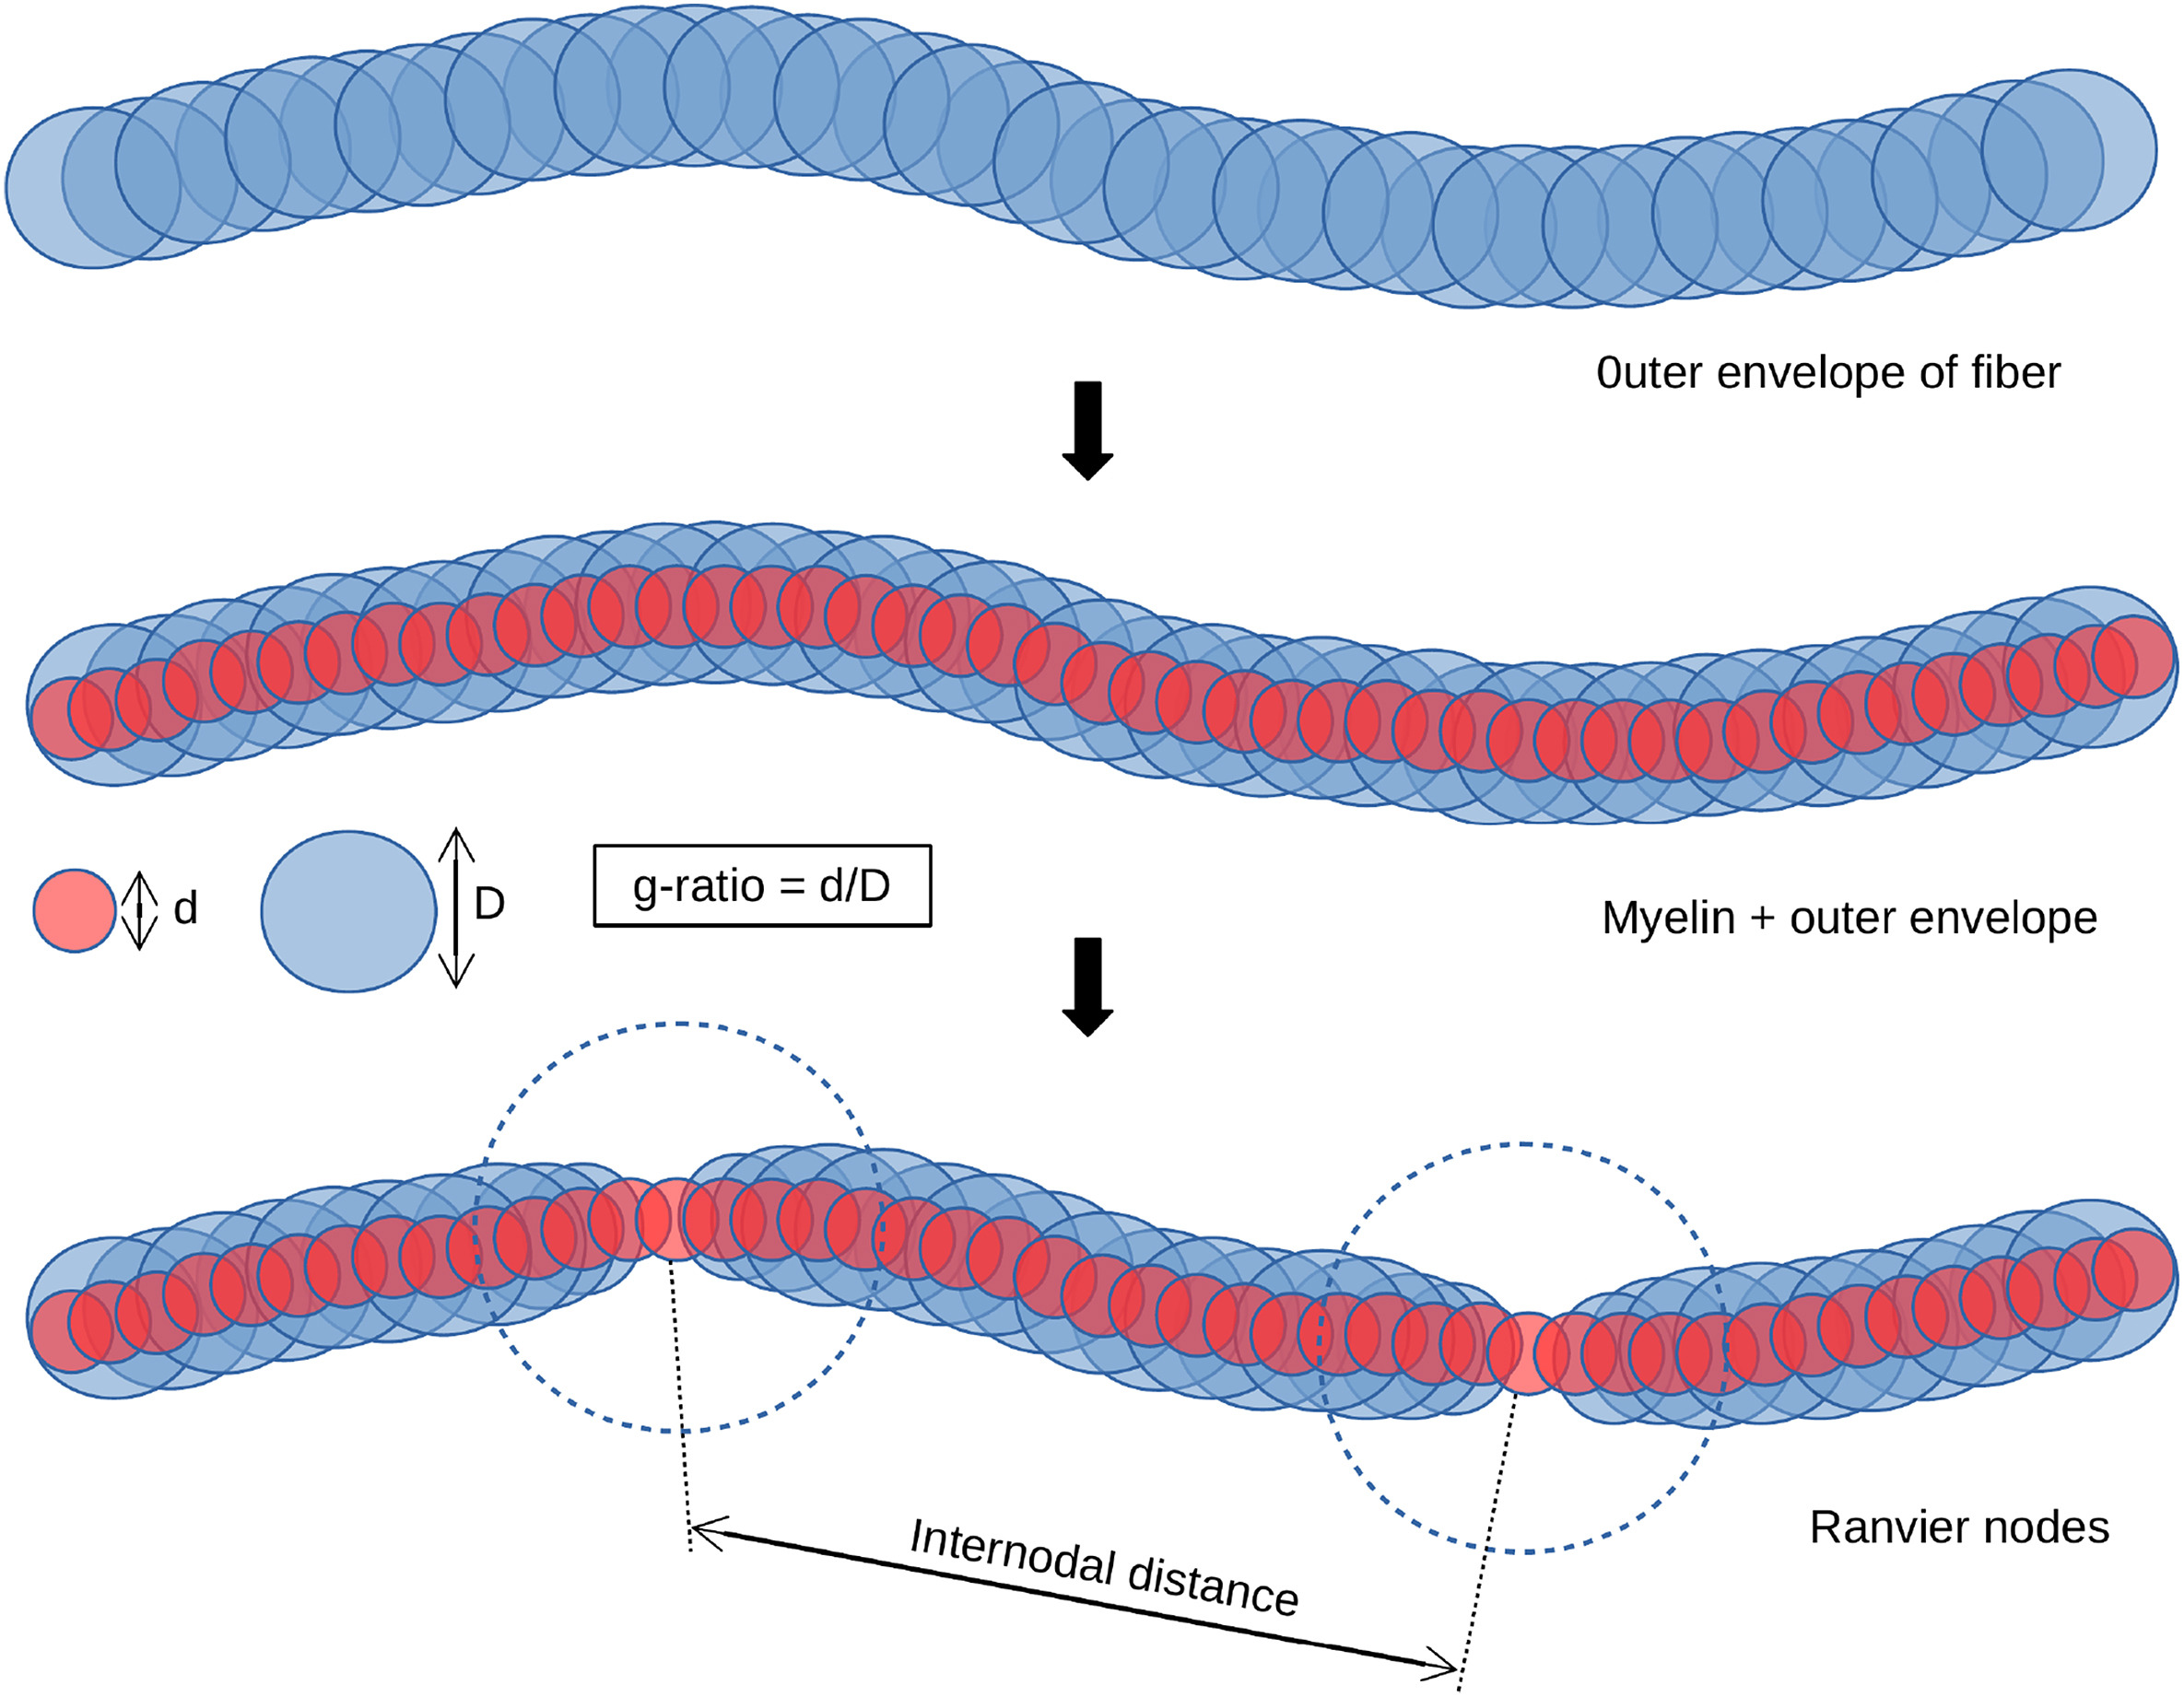
\includegraphics{gfx/model/medusa/4.jpg}
%     % }
% 	\caption{4 \cite{Ginsburger2019}}
% 	\label{fig:model:medusa_4_org}
% \end{figure}
% 
Since all objects are represented as a collection of spheres (see \cref{fig:model:medusa_4})
\begin{align}
    \mathcal{S} = \{ (x_i,y_i,z_i,r_i) : i \in \{0, 1, ..., n_\text{objects}-1\}  \} 
\end{align}
% 
, a collision is present if (VCS !!!)
% 
\begin{align}
\begin{split}
d<r_i+r_j\\
d = \abs{\vv{p}_i - \vv{p}_j}
\end{split}
\end{align}
% 
However since neighboring spheres in one fiber are colliding for a densly populated fiber, they have to be excluded if
\begin{align}
\begin{split}
d(i,j) &\leq  r_i + r_j\\
d(i,j) &= 
\begin{cases}
\sum_{n=i}^{j-1} \abs{\vv{p}_n - \vv{p}_{n+1}},& \text{if } j-i \geq 1\\
0 & \text{otherwise}
\end{cases}
\end{split}
\end{align}
% 
Spheres inside cell bodys are not checked for collision, since their volume aproximate? the volume of the cell.\\
% 
The calculation of collisions is done via the GPU architecture. For this a first implementation was written with the \name{AxisAligedSortedSearch} \cite{Karras2012}. It sorteds the spheres along one axis, \eg{} x-axis, x-axis, and search for each sphere the fist and last possible collision on this axis:
\begin{align}
\begin{split}
\mathcal{C}_i = \{ s \in \mathcal{S} \mid \abs{s_i.x - s_j.x} < r_i+r_j \}
\end{split}
\end{align}
% 
\begin{lstfloat}[!t]
	\lstinputlisting[style=cpp]{code/medusa.cu}
	\caption{Pseudocode of \acs{MEDUSA} collision checking.}
	\label{alg:medusa_collision}
\end{lstfloat}
% 
The above described algorithm is currently used for volumes $\approx \SI{200}{\micro\meter}$. For this volume size the algorithm is for the current use fast enough. However, more advaned algorithm exist wich can be applied here (\eg{} \name{BoundindBoxHierarchy} \cite{Karras2012}).
% 
\begin{figure}[!t]
    \centering
    \resizebox{0.95\textwidth}{!}{
    \includegraphics{gfx/model/medusa/8.jpg}}
	\caption{8 \cite{Ginsburger2019}}
	\label{fig:medusa_8}
\end{figure}
% 
\begin{figure}[!t]
    \centering
    \resizebox{0.95\textwidth}{!}{
    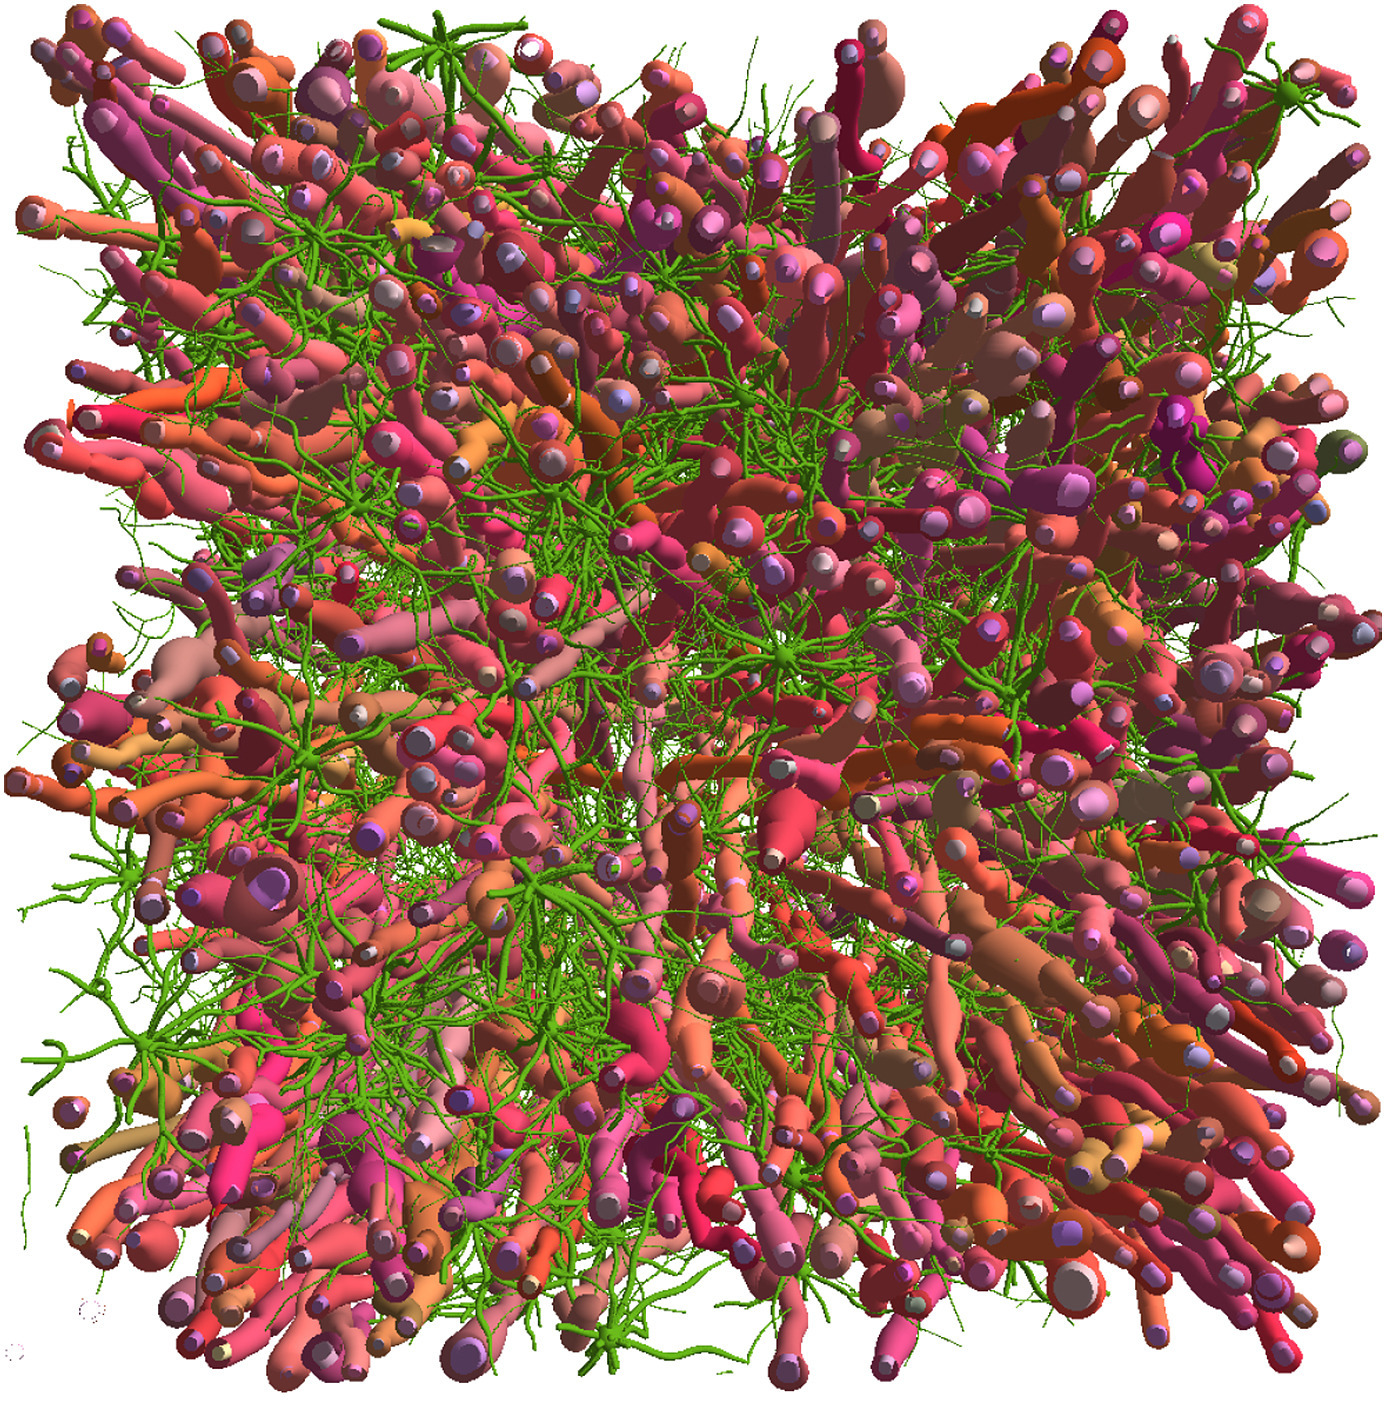
\includegraphics{gfx/model/medusa/11_.jpg}}
	\caption{11 \cite{Ginsburger2019}}
	\label{fig:medusa_11}
\end{figure}
% 
% 
% 
% 
% 
% 
% 
%
% Neurospin works with \ac{dMRI} signals.
% One focus is on the analysis of the fiber architect of the human brain.
% \ac{dMRI} is here quite handy since it is currently the only technique to allow in-vivo measurements to analyse the orientation of white matter tracts. Another importance is the availability of \ac{MRI} machines in almost every hospital in the western civilization.
% Although their resolution is with \SIrange{1.5}{3}{\tesla} limited.
% However, Neurospin is equipped with a mordern \SI{7}{\tesla} \ac{MRI}.
% This makes it possible, including higher measurments times on post mortem brain tissue, a \ac{dMRI} resolution up to \SI{200}{\micro\meter}.
% This makes it possible to allow \ac{3D-PLI} to verify and enhance the analysis of current developed tractography data. 
% %
% Along this works they developed a simulation tool (name) which is computing a Monte-Carlo simulation on the diffusion process in virtual tissues.
% Therefore, for simulations of the \ac{dMRI} signal in the brain, geometric models of nerve fibers as well as nerve cells are required.
% %
% The common goal was, due to a work packes inside the \ac{HBP}, the development of a common general purpose tool to build a geometrical library of nerve fiber configurations.
% Therefore it was decided to work based on the first approaches \cite{Ginsburger2018}.
% %
% \begin{quotation}
% We design a novel white matter numerical phantom generation algorithm which constructs biomimicking geometric configurations with few design parameters, and enables to control the level of disorder of the generated phantoms. The influence of various geometrical parameters present in white matter, such as global angular dispersion, tortuosity, presence of Ranvier nodes, beading, ...
% \end{quotation}
% %
% It is therefore qualified to generate a large database or library of parameter controlled white matter volumes.
% %
% \paragraph{differences:} 
% \begin{itemize}
%     \item All objects are aproximated with spheres.
%     \item Statistical ... of tissue
%     \item diffusion specific parameters
%     \item pathological changes like axon beeding
% \end{itemize}
% 
\section{"Conclusion"}
This allows a user to specify any initial configuration and reaching a collision free model, which, depending on the initial overlap, follows the initial geometry.
The disadvantage obvious is that the configuration has to change.
However since biological tissue is deformable and not "caotic" itself, it follows its natrual behavier.
